\documentclass[10pt]{article}
\usepackage[utf8]{inputenc}
\usepackage[T1]{fontenc}
\usepackage{amsmath}
\usepackage{amsfonts}
\usepackage{amssymb}
\usepackage[version=4]{mhchem}
\usepackage{stmaryrd}
\usepackage{graphicx}
\usepackage[export]{adjustbox}
\graphicspath{ {./images/} }
\usepackage{underscore}
\usepackage{bbold}
\usepackage{multirow}

\title{Finger trees: a simple general-purpose data structure }

\author{RALF HINZE\\
Institut für Informatik III, Universität Bonn\\
Römerstraße 164, 53117 Bonn, Germany\\
(e-mail: ralf@informatik.uni-bonn.de)\\
ROSS PATERSON\\
Department of Computing, City University\\
London EC1V OHB, UK\\
(e-mail: ross@soi.city.ac.uk)}
\date{}


\begin{document}
\maketitle


\begin{abstract}
We introduce 2-3 finger trees, a functional representation of persistent sequences supporting access to the ends in amortized constant time, and concatenation and splitting in time logarithmic in the size of the smaller piece. Representations achieving these bounds have appeared previously, but 2-3 finger trees are much simpler, as are the operations on them. Further, by defining the split operation in a general form, we obtain a general purpose data structure that can serve as a sequence, priority queue, search tree, priority search queue and more.
\end{abstract}

\section*{1 Introduction}
Lists are the functional programmer's favourite data type. They are well supported by most if not all functional programming languages. However, one could argue that this support sometimes leads programmers to use lists when a more general sequence type would be more appropriate (Okasaki, 2000). The operations one might expect from a sequence abstraction include adding and removing elements at both ends (the deque operations), concatenation, insertion and deletion at arbitrary points, finding an element satisfying some criterion, and splitting the sequence into subsequences based on some property. Many efficient functional implementations of subsets of these operations are known, but supporting more operations efficiently is difficult. The best known general implementations are very complex, and little used.

This paper introduces functional 2-3 finger trees, a general implementation that performs well, but is much simpler than previous implementations with similar bounds. The data structure and its many variations are simple enough that we are able to give a concise yet complete executable description using the functional programming language Haskell (Peyton Jones, 2003). The paper should be accessible to anyone with a basic knowledge of Haskell and its widely used extension to\\
multiple-parameter type classes (Peyton Jones et al., 1997). Although the structure makes essential use of laziness, it is also suitable for strict languages that provide a lazy evaluation primitive.

The rest of the paper is organized as follows. The next section contains some preliminary material used throughout the paper. In Section 3 we describe the finger tree type, an elegant example of a first-order nested type, and show how it supports deque operations and concatenation. In Section 4 we define a variation of the finger tree type that supports a splitting operation, abstracting over the annotation used to guide splitting. In this way we obtain a general purpose data structure that can serve as a sequence, priority queue, search tree, priority search queue and more. Moreover, these trees perform well in each role, though specialized implementations are usually faster. Section 5 concludes, including a discussion of related work.

We have included several exercises to support the digestion of the material and to discuss further variations and extensions.

\section*{2 Preliminaries}
This section briefly reviews two fundamental concepts, monoids and reductions, that are at the heart of the later development.

\subsection*{2.1 Monoids}
A type with an associative operation and an identity forms a monoid.

$$
\begin{aligned}
& \text { class Monoid } a \text { where } \\
& \quad \emptyset \quad:: a \\
& \quad(\oplus):: a \rightarrow a \rightarrow a
\end{aligned}
$$

We shall introduce a variety of monoids later on.\\
A single type is sometimes the carrier of several different monoids. In this case, we will introduce an isomorphic type via a newtype declaration for each monoidal structure of interest.

\subsection*{2.2 Right and left reductions}
Monoids are often used with reductions. A reduction is a function that collapses a structure of type $f a$ into a single value of type $a$ (Meertens, 1996): empty subtrees are replaced by a constant, such as $\emptyset$; intermediate results are combined using a binary operation, such as ' $\oplus$ '. A reduction with a monoid yields the same result however we nest the applications of ' $\oplus$ ', but for a reduction with an arbitrary constant and binary operation we must specify a particular nesting. If we arrange that applications of the combining operation are only nested to the right, or to the left, then we obtain skewed reductions, which we single out as a type class.

\begin{verbatim}
class Reduce f where
    reducer :: (a->b->b)->(fa->b->b)
    reducel :: (b->a->b) ->(b->fa->b)
\end{verbatim}

Skewed reductions are far more general than reductions: they not only take an arbitrary binary operation and an arbitrary element, the arguments of the binary operation may even have different types.

The order of reducer's parameters is arranged as to suggest an alternative reading: reducer $(\prec)$ lifts the operation ' $\prec$ ' to $f$-structures. As an example, if ' $\prec$ ' adds an element to a container, then reducer $(\prec)$ adds a complete $f$-structure.

Skewed reductions need not be written by hand; they can be defined generically for arbitrary $f$-structures (Hinze \& Jeuring, 2003). Nonetheless, we shall provide all the necessary instances in order to keep the paper self-contained.

On lists, reductions specialize to folds.

\begin{verbatim}
instance Reduce [] where
    reducer (<)xz= foldr ( <) zx -- NB. x and z are swapped
    reducel ( }\succ)xz=\mathrm{ foldl ( }\succ\mathrm{ ) xz
\end{verbatim}

Reductions are particularly useful for converting between structures.

\begin{verbatim}
toList $\quad::($ Reduce $f) \Rightarrow f a \rightarrow[a]$
toList $s=s:$ ' [] where $\left(:^{\prime}\right)=\operatorname{reducer}(:)$
\end{verbatim}

Think of the structure $s$ as being cons'ed to the empty list.

\section*{3 Simple sequences}
We first develop the definition of 2-3 finger trees, and then show how they efficiently implement sequences. As a starting point, consider ordinary 2-3 trees, like the one below:\\
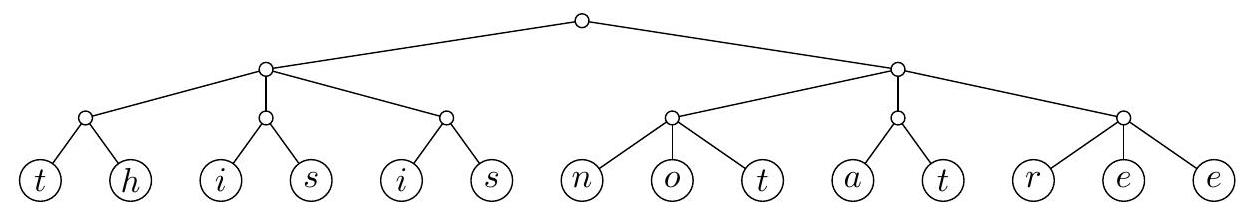
\includegraphics[max width=\textwidth, center]{2025_02_02_ca76fc9910387742713ag-03}

The structural constraint that all leaves occur at the same level may be expressed by defining a non-regular or nested type (Bird \& Meertens, 1998), as follows:

\begin{verbatim}
data Tree a = Zero a Succ (Tree (Node a))
data Node a = Node2 a a | Node3 a a a
\end{verbatim}

Values of type Tree $a$ have the form Succ $^{n}$ (Zero $t$ ) for some $n$, where $t$ has type Node ${ }^{n} a$, the type of well-formed 2-3 trees of depth $n$. Note that the internal nodes of these trees contain no keys; in this section we shall store all data in the leaves of our trees.

Operations on such trees typically take time logarithmic in the size of the tree, but for a sequence implementation we would like to add and remove elements from either end in constant time.

\subsection*{3.1 Finger trees}
A structure providing efficient access to nodes of a tree near a distinguished location is called a finger (Guibas et al., 1977). In an imperative setting, this would be done by reversing pointers. In a functional setting, we can transform the structure in a manner reminiscent of Huet's "zipper" structure (1997).

To provide efficient access to the ends of a sequence, we wish to place fingers at the left and right ends of this tree. Imagine taking hold of the end nodes of the example tree above and lifting them up together. We would obtain a tree that looks like this:\\
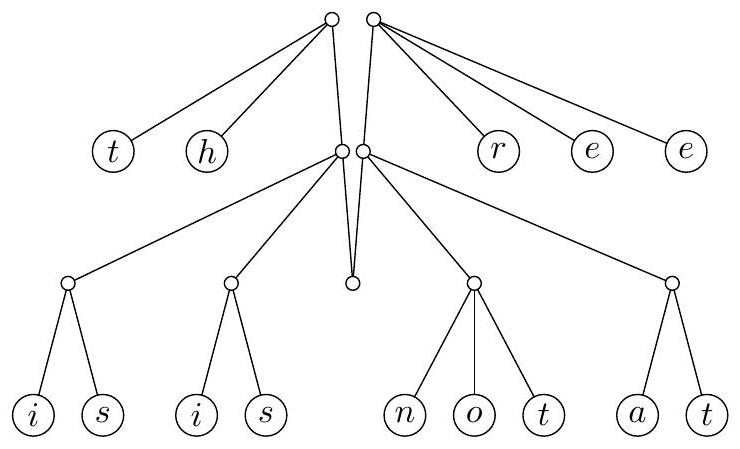
\includegraphics[max width=\textwidth, center]{2025_02_02_ca76fc9910387742713ag-04}

Because all leaves of the original 2-3 tree were at the same depth, the left and right spines have the same length, and we can pair corresponding nodes on these spines to make a single central spine. Hanging off the sides of these nodes are 2-3 trees, whose depth increases as we descend the central spine. The first level contains two or three elements on each side, while the others have one or two subtrees. At the bottom of the spine, we have either a single 2-3 tree or none, depending on whether the old root had a degree of 3 or 2 . We can describe this structure as follows:

$$
\begin{aligned}
\text { data FingerTree } a & =\text { Empty } \\
& \mid \text { Single a } \\
& \mid \text { Deep }(\text { Digit a) }(\text { FingerTree }(\text { Node a) })(\text { Digit a) }
\end{aligned}
$$

where a digit is a buffer of elements stored left to right (in the picture digits are depicted by filled circles), here represented as a list to simplify the presentation:

$$
\text { type Digit } a=[a]
$$

As noted above, in transformed 2-3 trees these lists have length 2 or 3 at the top level and 1 or 2 at lower levels. We shall relax this, allowing between one and four subtrees at each level. As we shall see in the next subsection, this relaxation provides just enough slack to buffer deque operations efficiently. By the way, the buffer type is called Digit because finger trees are a so-called numerical representation (Okasaki, 1998), a data structure that is modelled after a number system.

The non-regular definition of the FingerTree type determines the unusual shape of these trees, which is the key to their performance. The top level contains elements of type $a$, the next of type Node $a$, and so on: the $n$th level contains elements of type Node ${ }^{n} a$, namely 2-3 trees of depth $n$. Thus a sequence of $n$ elements is represented\\
by a tree of depth $\Theta(\log n)$. Moreover, an element $d$ positions from the nearest end is stored at a depth of $\Theta(\log d)$ in the tree.

Before moving on, we instantiate the generic definition of reduction to these types. Reduction of nodes is trivial:

\begin{verbatim}
instance Reduce Node where
    reducer ( }<)(\mathrm{ Node2 a b) z=a}\prec(b\precz
    reducer ( <) (Node3 a b c) z=a\prec(b\prec(c\precz))
    reducel (>) z (Node2 b a) = (z\succb)\succa
    reducel }(\succ)z(Node3 c b a)=((z\succc)\succb)\succ
\end{verbatim}

Reduction of finger trees uses single and double liftings of the binary operation:

\begin{verbatim}
instance Reduce FingerTree where
    reducer $(\prec)$ Empty $\quad z=z$
    reducer $(\prec)($ Single $x) \quad z=x \prec z$
    reducer $(\prec)($ Deep pr $m s f) z=p r \prec^{\prime}\left(m \prec^{\prime \prime}\left(s f \prec^{\prime} z\right)\right)$
        where $\left(\prec^{\prime}\right)=$ reducer $(\prec)$
            $\left(\prec^{\prime \prime}\right)=$ reducer $($ reducer $(\prec))$
    reducel $(\succ) z$ Empty $=z$
    reducel $(\succ) z$ (Single $x)=z \succ x$
    reducel $(\succ) z($ Deep pr $m s f)=\left(\left(z \succ^{\prime} p r\right) \succ^{\prime \prime} m\right) \succ^{\prime} s f$
        where $\left(\succ^{\prime}\right)=$ reducel $(\succ)$
            $\left(\succ^{\prime \prime}\right)=\operatorname{reducel}(\operatorname{reducel}(\succ))$
\end{verbatim}

\subsection*{3.2 Deque operations}
We shall now proceed to show that finger trees make efficient deques, with all operations taking $\Theta(1)$ amortized time. This holds even if the structure is used in a persistent manner, where several versions of a tree may coexist (Driscoll et al., 1989). The analysis is essentially the same as that for Okasaki's implicit deques (1998). Indeed, the FingerTree type differs from implicit deques primarily in storing Nodes instead of pairs, with a corresponding increase in the size of digits. This change provides the necessary flexibility for efficient implementation of concatenation and splitting, as we shall see later.

Adding a new element to the left of the sequence is trivial, except when the initial buffer already contains four elements. In that case, we push three of the elements as a Node, leaving two behind:

\section*{infixr $5 \triangleleft$}
$$
\begin{array}{ll}
(\triangleleft) & :: ~ a \rightarrow \text { FingerTree } a \rightarrow \text { FingerTree a } \\
a \triangleleft \text { Empty } & =\text { Single } a \\
a \triangleleft \text { Single } b & \\
a \triangleleft \text { Deep }[a] \text { Empty }[b] \\
a \triangleleft \text { Deep }[b, d, e] m s f & =\text { Deep }[a, b](\text { Node3 } c d e \triangleleft m) s f \\
a \triangleleft \text { Deep pr msf } & =\text { Deep }([a]+p r) m \text { sf }
\end{array}
$$

The function ' $\triangleleft$ ' requires a non-schematic form of recursion, called polymorphic\\
recursion (Mycroft, 1984): the recursive call adds a node (not an element) to a finger tree that contains Nodes.

Adding to the right end of the sequence is the mirror image of the above:\\
infixl $5 \triangleright$\\
$(\triangleright) \quad::$ FingerTree $a \rightarrow a \rightarrow$ FingerTree $a$\\
Empty $\triangleright a=$ Single $a$\\
Single $b \quad \triangleright a=$ Deep $[b]$ Empty $[a]$\\
Deep pr $m[e, d, c, b] \triangleright a=$ Deep pr $(m \triangleright N o d e 3$ e $d c)[b, a]$\\
Deep prmsf $\quad \triangleright a=$ Deep pr $m(s f+[a])$\\
We shall also require the liftings of ' $\triangleleft$ ' and ' $\triangleright$ ':\\
$\left(\triangleleft^{\prime}\right)::($ Reduce $f) \Rightarrow f a \rightarrow$ FingerTree $a \rightarrow$ FingerTree $a$\\
$\left(\triangleleft^{\prime}\right)=\operatorname{reducer}(\triangleleft)$\\
$\left(\triangleright^{\prime}\right)::($ Reduce $f) \Rightarrow$ FingerTree $a \rightarrow f a \rightarrow$ FingerTree $a$\\
$\left(\triangleright^{\prime}\right)=$ reducel $(\triangleright)$\\
Conversion to a finger tree may be defined using either ' $\triangleleft^{\prime}$ ' or ' $\nabla^{\prime}$ '; we use the former:

$$
\begin{aligned}
& \text { toTree }::(\text { Reduce } f) \Rightarrow f a \rightarrow \text { FingerTree } a \\
& \text { toTree } s=s \triangleleft^{\prime} \text { Empty }
\end{aligned}
$$

To deconstruct a sequence, we define a type that expresses a view of the left end of a sequence as either empty or an element together with the rest of the sequence:

$$
\operatorname{data}_{V i e w_{L}} \text { s } a=\operatorname{Nil}_{L} \left\lvert\, \operatorname{Cons}_{L} a\left(\begin{array}{ll}
s & a
\end{array}\right)\right.
$$

The left view of a sequence maps a sequence to this type:

$$
\begin{array}{ll}
\text { view }_{L} & :: \text { FingerTree } a \rightarrow \text { View }_{L} \text { FingerTree a } \\
\text { view }_{L} \text { Empty } & =\text { Nil }_{L} \\
\text { view }_{L}(\text { Single } x) & =\text { Cons }_{L} \times \text { Empty } \\
\text { view }_{L}(\text { Deep pr } m \text { sf }) & =\text { Cons }_{L}(\text { head pr })\left(\text { deep }_{L}(\text { tail pr }) m \text { sf }\right)
\end{array}
$$

Since the prefix pr of a Deep tree contains at least one element, we can get its head in constant time. However, the tail of the prefix may be empty, and thus unsuitable as a first argument to the Deep constructor. Hence we define a smart constructor that differs from Deep by allowing the prefix to contain zero to four elements, and in the empty case uses a left view of the middle tree to construct a tree of the correct shape:

$$
\begin{aligned}
& \text { deep } \left._{L} \quad::[a] \rightarrow \text { FingerTree (Node } a\right) \rightarrow \text { Digit } a \rightarrow \text { FingerTree } a \\
& \text { deep }_{L}[] m \text { sf }=\text { case } \operatorname{view}_{L} m \text { of } \\
& \text { Nil }_{L} \quad \rightarrow \text { toTree sf } \\
& \text { Cons }_{L} \text { a } m^{\prime} \rightarrow \text { Deep (toList a) } m^{\prime} \text { sf } \\
& \text { deep }_{L} \text { pr } m s f=\text { Deep pr } m s f
\end{aligned}
$$

Then we can define separate functions isEmpty, head $_{L}$, and tail $_{L}$ using the view:

\begin{verbatim}
isEmpty :: FingerTree $a \rightarrow$ Bool
isEmpty $x=$ case view $_{L} x$ of $N i l_{L} \quad \rightarrow$ True
                                    Cons $_{L}-\mathbf{} \rightarrow$ False
head $_{L} \quad::$ FingerTree $a \rightarrow a$
$\operatorname{head}_{L} x=$ case view $_{L} x$ of $\operatorname{Cons}_{L} a-\rightarrow a$
tail $_{L} \quad::$ FingerTree $a \rightarrow$ FingerTree $a$
$\operatorname{tail}_{L} x=$ case view $_{L} x$ of $\operatorname{Cons}_{L}-x^{\prime} \rightarrow x^{\prime}$
\end{verbatim}

In a lazy language like Haskell, the tail part of the view is not computed unless it is used. In a strict language, it might be more useful to provide the three separate functions as primitives.

We omit the code for the right view, which is a mirror image of the left view, including a function deep $_{R}$ corresponding to deep $L_{L}$.

Each deque operation may recurse down the spine of the finger tree, and thus take $\Theta(\log n)$ time in the worst case. However, it can be shown that these operations take only $\Theta(1)$ amortized time, even in a persistent setting. The analysis is essentially the same as Okasaki's for implicit deques (Okasaki, 1998). We outline the main points here.

We classify digits of two or three elements (which are isomorphic to elements of type Node a) as safe, and those of one or four elements as dangerous. A deque operation may only propagate to the next level from a dangerous digit, but in doing so it makes that digit safe, so that the next operation to reach that digit will not propagate. Thus, at most half of the operations descend one level, at most a quarter two levels, and so on. Consequently, in a sequence of operations, the average cost is constant.

The same bounds hold in a persistent setting if subtrees are suspended using lazy evaluation. This ensures that transformations deep in the spine do not take place until a subsequent operation needs to go down that far. Because of the above properties of safe and dangerous digits, by that time enough cheap shallow operations will have been performed to pay for this expensive evaluation.

This argument may be formalized using Okasaki's debit analysis (1998) by assigning the suspension of the middle tree in each Deep node as many debits as the node has safe digits. (It may have 0,1 or 2.) A deque operation that descends $k$ levels turns $k$ dangerous digits into safe ones, and thus creates $k$ debits to pay for the work involved. Applying Okasaki's technique of debit passing to any debits already attached to these $k$ nodes, one can show that each operation must discharge at most one debit, so the deque operations run in $\Theta(1)$ amortized time.

Lazy evaluation is the norm in a language such as Haskell. In a strict language that provides a lazy evaluation primitive, we need only suspend the middle subtree of each Deep node, so only $\Theta(\log n)$ suspensions are required in a tree of size $n$. Even in a lazy language, some space could be saved in practice by ensuring that these were the only suspensions in the tree, for example by using Haskell's strictness annotations. Indeed we might wish to make the operations even more strict, for example by forcing the middle subtree $m$ in the recursive case of ' $\triangleleft$ ' to avoid building\\
a chain of suspensions. According to the above debit analysis, this suspension has been paid for by this time, so the amortized bounds would be unaffected.

While we chose to push a Node3 in ' $\triangleleft$ ' and ' $\triangleright$ ', leaving two elements behind, pushing a Node2 instead also yields the same bounds. Our choice means that the tree is mostly populated with nodes of degree 3 , and therefore slightly shallower. It is also faster in queue-like applications, where elements are mostly added at one end and mostly removed from the other, because it means that only every third operation propagates to the next level.\\
Exercise 1. In the above presentation, we represented digits as lists for simplicity. A more accurate and efficient implementation would use the type

\begin{verbatim}
data Digit a = One a
    | Two a a
    | Three a a a
    | Four a a a a
\end{verbatim}

Rework the above definitions to use this definition of Digit.

\subsection*{3.3 Concatenation}
We now consider concatenation of sequences represented as finger trees. The tree Empty will be an identity for concatenation, and concatenation with Singles reduces to ' $\triangleleft$ ' or ' $\triangleright$ ', so the only difficult case is concatenation of two Deep trees. We can use the prefix of the first tree as the prefix of the result, and the suffix of the second tree as the suffix of the result. To combine the rest to make the new middle subtree, we require a function of type

$$
\begin{aligned}
& \text { FingerTree }(\text { Node } a) \rightarrow \text { Digit } a \rightarrow \text { Digit } a \rightarrow \text { FingerTree }(\text { Node } a) \rightarrow \\
& \quad \text { FingerTree }(\text { Node } a)
\end{aligned}
$$

Since it is easy to combine the two digit arguments into a list of Nodes, we can obtain a recursive function by generalizing the concatenation function to take an additional list of elements:

\begin{verbatim}
app3 :: FingerTree }a->[a]->\mathrm{ FingerTree a }->\mathrm{ FingerTree a
app3 Empty ts xs = ts \triangleleft' xs
app3 xs ts Empty = xs \triangleright
app3 (Single x) ts xs=x\triangleleft(ts \triangleleft' xs)
app3 xs ts (Single x)=(xs\mp@subsup{\triangleright}{}{\prime}ts)\trianglerightx
app3 (Deep pr r m m sf 1) ts (Deep pr 2 m m sf 2)
\end{verbatim}

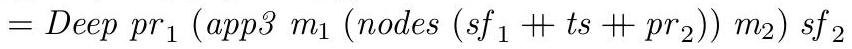
\includegraphics[max width=\textwidth, center]{2025_02_02_ca76fc9910387742713ag-08}\\
where ' $\triangleleft$ ' and ' $\triangleright$ ' are the previously defined liftings of ' $\triangleleft$ ' and ' $\triangleright$ ', and nodes groups a list of elements into Nodes:

\begin{verbatim}
nodes :: [a] ->[Node a]
nodes [a,b] = [Node2 a b]
nodes [a,b,c] =[Node3 a b c]
nodes [a,b,c,d] =[Node2 a b,Node2 c d]
nodes (a:b:c:xs)=Node3 a b c:nodes xs
\end{verbatim}

Now we can concatenate two finger trees by starting with an empty list between them:

$$
\begin{aligned}
& (\bowtie) \quad:: \text { FingerTree } a \rightarrow \text { FingerTree } a \rightarrow \text { FingerTree } a \\
& x s \bowtie y s=\text { app3 xs [] ys }
\end{aligned}
$$

It is easy to check that in each of the invocations of app3 arising from ' $\bowtie$ ', the list argument has length at most 4 , so each of these invocations takes $\Theta(1)$ time. The recursion terminates when we reach the bottom of the shallower tree, with up to 4 insertions, so the total time taken is $\Theta\left(\log \left(\min \left\{n_{1}, n_{2}\right\}\right)\right)$, where $n_{1}$ and $n_{2}$ are the numbers of elements in the argument trees.

Note that the debit analysis of Section 3.2 remains valid, because although ' $\bowtie$ ' must discharge any debits on the nodes on the spines that are merged, there will be at most $\Theta\left(\log \left(\min \left\{n_{1}, n_{2}\right\}\right)\right)$ of these.\\
Exercise 2. The definition of nodes prefers to use Node3 where possible, but any other choices would still yield the same asymptotic bounds. If nodes were redefined to prefer Node2, what would be the bound on the length of the list arguments in the invocations of app3 arising from ' $\bowtie$ '?\\
Exercise 3. Consider replacing the Digit type as discussed in Exercise 1, and also using a variant of app3 for each possible size of the middle argument. This leads to a faster but much larger definition. Hint: it is both simpler and less error-prone to write a program that generates the Haskell source for this definition.

\section*{4 Annotated sequences}
Finger trees serve remarkably well as implementations of catenable deques. In this section we shall present a modification of these trees, which also provides positional and set-theoretic operations, such as taking or dropping the first $n$ elements of a sequence or partitioning an ordered sequence around a pivot element.

As a common characteristic, all of these operations involve searching for an element with a certain property. For example, partitioning an ordered sequence involves searching for the minimum element that is larger than or equal to the pivot element. Thus, if we want to implement the additional operations with reasonable efficiency, we must be able to steer this search. To this end we augment the internal nodes of a finger tree by an additional field that contains positional or ordering information or both.

\subsection*{4.1 Measurements}
We take the fairly liberal view that an annotation represents a cached reduction with some monoid. Reductions, possibly cached, are captured by the following class declaration (for clarity, we use mixfix notation, which is not possible in Haskell).

\begin{verbatim}
class $($ Monoid $v) \Rightarrow$ Measured $a v$ where
    $\|\cdot\|:: a \rightarrow v$
\end{verbatim}

Think of $a$ as the type of some tree and $v$ as the type of an associated measurement. As customary, $v$ must possess a monoidal structure so that we can easily\\
combine measurements of subtrees independent of their nesting. For instance, the 'size' measure maps onto the monoid of natural numbers with addition. In this particular example, the binary operation is not only associative but also commutative, but this need not be the case in general.

The class Measured is parameterized by both $a$ and $v$ and represents a true many-to-many relation on types: the same measurement may be imposed on a variety of types; the same type may be measured in many different ways. Unfortunately, this means that the class declaration is not legal Haskell 98, which only admits singleparameter type classes. Multiple parameter classes (Peyton Jones et al., 1997), however, are supported as an extension by the most widely used Haskell implementations.

\subsection*{4.2 Caching measurements}
Obtaining a measure should be cheap. We shall ensure that finger trees support this operation with a bounded number of ' $\oplus$ ' operations. To this end we cache measurements in 2-3 nodes.

$$
\text { data Node } v a=\text { Node2 } v a \operatorname{a} \mid \text { Node3 } v a \operatorname{a} a
$$

The smart constructors node2 and node3 automatically add an explicit annotation

$$
\begin{array}{ll}
\text { node2 } & ::(\text { Measured } a v) \Rightarrow a \rightarrow a \rightarrow \text { Node } v a \\
\text { node2 } a b & =\text { Node2 }(\|a\| \oplus\|b\|) a b \\
\text { node3 } & ::(\text { Measured } a v) \Rightarrow a \rightarrow a \rightarrow a \rightarrow \text { Node } v a \\
\text { node3 } a b c & =\text { Node3 }(\|a\| \oplus\|b\| \oplus\|c\|) a b c
\end{array}
$$

This annotation is then retrieved by the measure function:

$$
\begin{aligned}
& \text { instance }(\text { Monoid } v) \Rightarrow \text { Measured }(\text { Node } v a) v \text { where } \\
& \| \text { Node2 } v--\|=v \\
& \| \text { Node3 } v---\|=v
\end{aligned}
$$

The smart constructors and the instance declaration are completely generic: they work for arbitrary annotations.

Digits are measured on the fly.

$$
\begin{aligned}
& \text { instance (Measured a } v) \Rightarrow \text { Measured (Digit a) } v \text { where } \\
& \quad\|x s\|=\operatorname{reducel}(\lambda i a \rightarrow i \oplus\|a\|) \emptyset \text { xs }
\end{aligned}
$$

Recall that a digit is a buffer of one to four elements. Because the length of the buffer is bounded by a constant, the number of ' $\oplus$ ' operations is also bounded. Another possibility is to cache the measure of a digit, adding to the cost of digit construction but yielding a saving when computing the measure. The choice between these strategies would depend on the expected balance of query and modification operations, but they would differ only by a constant factor.

Finger trees are modified in a similar manner to 2-3 nodes. Again there is a choice of caching strategies, but it suffices to cache deep nodes:

\section*{data FingerTree $v a=$ Empty}
| Single a\\
| Deep v (Digit a) (FingerTree v (Node va)) (Digit a)\\
The top level of an annotated finger tree contains elements of type $a$, the second level of type Node $v a$, the third of type Node $v$ (Node $v a$ ), and so on. Whereas the tree type $a$ changes from level to level, the annotation type $v$ remains the same. In a nutshell, FingerTree is nested in $a$, but regular in $v$.

Again, a smart constructor takes care of filling in the missing annotation

$$
\begin{aligned}
& \text { deep }::(\text { Measured a } v) \Rightarrow \\
& \quad \text { Digit } a \rightarrow \text { FingerTree } v(\text { Node } v a) \rightarrow \text { Digit } a \rightarrow \text { FingerTree } v a \\
& \text { deep pr } m \text { sf }=\text { Deep }(\|p r\| \oplus\|m\| \oplus\|s f\|) \text { pr m sf }
\end{aligned}
$$

This annotation is then available for subsequent measurements:

$$
\begin{aligned}
& \text { instance (Measured a } v) \Rightarrow \text { Measured (FingerTree } v \text { a) } v \text { where } \\
& \begin{aligned}
\| \text { Empty } \| & =\emptyset \\
\| \text { Single } x \| & =\|x\| \\
\| \text { Deep } v---\| & =v
\end{aligned}
\end{aligned}
$$

\subsection*{4.3 Construction, deconstruction and concatenation}
None of the sequence operations introduced in Section 3 benefits from the annotations. Consequently, their re-implementations can simply ignore the additional field in pattern matching and recompute it when constructing nodes. The latter is most easily accomplished by replacing the original constructors by their smart counterparts (in expressions). The re-implementation of ' $\triangleleft$ ' illustrates the necessary amendments:

$$
\begin{aligned}
& \text { infixr } 5 \triangleleft \\
& (\triangleleft)::(\text { Measured } a v) \Rightarrow a \rightarrow \text { FingerTree } v a \rightarrow \text { FingerTree } v a \\
& a \triangleleft \text { Empty } \quad=\text { Single } a \\
& a \triangleleft \text { Single } b \quad=\text { deep }[a] \text { Empty }[b] \\
& a \triangleleft \text { Deep } \quad[b, c, d, e] m s f=\operatorname{deep}[a, b](\text { node3 } c d e \triangleleft m) s f \\
& a \triangleleft \text { Deep _prmsf } \quad=\operatorname{deep}([a]+p r) m s f
\end{aligned}
$$

The remaining operations are changed accordingly. Their time bounds remain as in Section 3, except that they now refer to the number of ' $\oplus$ ' operations required to compute the new annotations.

\subsection*{4.4 Splitting}
A scan is an iterated reduction that maps the sequence $x_{1}, \ldots, x_{n}$ of elements to the sequence $v_{1}, \ldots, v_{n}$ of accumulated measurements where $v_{j}=i \oplus\left\|x_{1}\right\| \oplus \cdots \oplus\left\|x_{j}\right\|$ for some start value $i$. The next operation we introduce will use the annotations to efficiently split a sequence based on properties of the scan with the monoid. For instance, a 'size' scan yields the positions of elements so that we can split a sequence at a given position. Since ' $\oplus$ ' is associative, a scan can be calculated on the fly using the cached reductions in the nodes.

To represent a container split around a distinguished element, with containers of elements to its left and right, we introduce the data type

\begin{verbatim}
data Split fa=Split (f a) a (fa)
\end{verbatim}

The Split type singles out an element and its context, in a similar way to a finger in an imperative setting or a zipper in a functional setting. Splitting a finger tree provides us with a third finger besides the ones at the left and right ends of the tree.

The function splitTree, which splits a finger tree, expects three arguments: a predicate $p$ on measurements, an accumulator $i$, and a finger tree $t$. It is specified

$$
\begin{aligned}
\neg p i \wedge p(i \oplus\|t\|) \Longrightarrow & \\
\text { let Split } l x r=\text { splitTree } p \text { it in } & \text { toList } l+[x]+\text { toList } r=\text { toList } t \\
& \wedge \neg p(i \oplus\|l\|) \wedge p(i \oplus\|l\| \oplus\|x\|)
\end{aligned}
$$

The first conjunct states that Split $l x r$ is actually a split of $t$, that is, the order and multiplicity of elements is preserved. As usual for this type of condition, it will be fairly obvious from the program text that the property is satisfied. Indeed, we take great care that the relative order of elements is preserved in the syntax of our code.

The other conjunct states that splitTree splits $t$ at a point where $p$ applied to the accumulated measurement changes from False to True. The precondition expresses that this measurement is False at the left end and True at the right end, so there is at least one such point. The precondition implies, in particular, that $t$ is non-empty. Splitting is most useful if there is exactly one such point, but we need not assume this. Uniqueness of the split is guaranteed for monotonic predicates satisfying $p x \Longrightarrow p(x \oplus y)$ or equivalently $\neg p(x \oplus y) \Longrightarrow \neg p x$ for all $x$ and $y$. Alternatively, an application might maintain an invariant on sequences that guarantees a unique split for predicates of interest; Section 4.7 provides an example of this.

The picture below illustrates the functioning of splitTree.\\
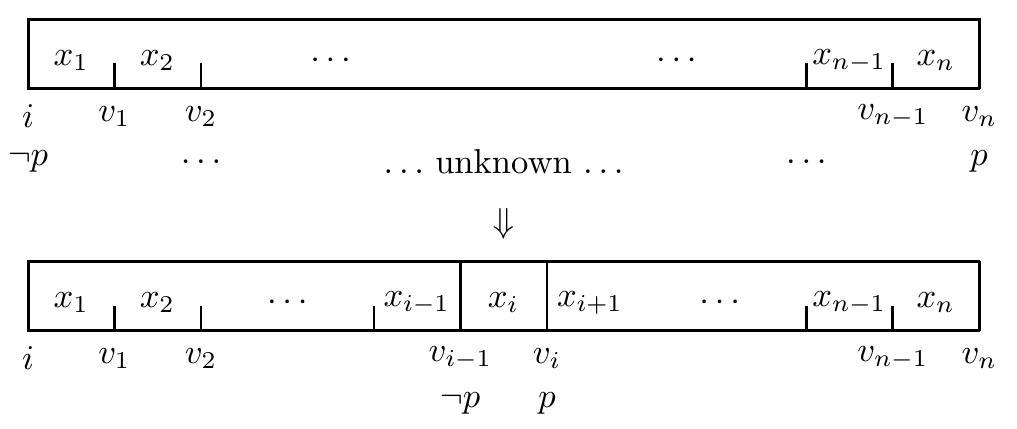
\includegraphics[max width=\textwidth, center]{2025_02_02_ca76fc9910387742713ag-12}\\
where $v_{j}=i \oplus\left\|x_{1}\right\| \oplus \cdots \oplus\left\|x_{j}\right\|$. In the diagram, $x_{i}$ is the distinguished element where $p$ changes from False to True.

The helper function splitDigit, which satisfies an analogous specification, nicely illustrates splitting along a scan.

\begin{verbatim}
splitDigit $::($ Measured $a v) \Rightarrow(v \rightarrow$ Bool $) \rightarrow v \rightarrow$ Digit $a \rightarrow$ Split [] a
splitDigit $p i[a]=\operatorname{Split}[] a[]$
splitDigit $p i(a: a s)$
    $\mid p i^{\prime}=$ Split [] a as
    $\mid$ otherwise $=$ let Split $l x r=$ splitDigit $p i^{\prime}$ as in Split $(a: l) x r$
    where $i^{\prime}=i \oplus\|a\|$
\end{verbatim}

The type signature makes precise that splitting a digit may produce empty left and right buffers ('[]' is the list type constructor). The reader is invited to check that the invariant expressed in the specification is indeed preserved through the recursive calls. Since splitDigit scans the list from left to right, it actually splits the list at the first point where $p$ flips. The function splitTree proceeds in a similar fashion, but it may skip whole subtrees (which become deeper as we descend the tree). This behaviour is necessary to make splitTree run in logarithmic time, but it also means that there is no guarantee that the calculated split is the first one. The definition of splitTree uses the auxiliary function deep $_{L}$ from Section 3.2 and its mirror image deep $_{R}$.

\begin{verbatim}
splitTree :: (Measured a $v$ ) $\Rightarrow$
    $(v \rightarrow$ Bool $) \rightarrow v \rightarrow$ FingerTree $v a \rightarrow$ Split (FingerTree $v) a$
splitTree pi(Single $x)=$ Split Empty $x$ Empty
splitTree pi(Deep_prmsf)
    $\mid p$ vpr $\quad=$ let Split $l x r=$ splitDigit $p$ i pr
                        in Split (toTree l) $x\left(\right.$ deep $\left._{L} r m s f\right)$
    $\mid p \mathrm{vm}=$ let Split ml xs mr $=$ splitTree $p \mathrm{vpr} m$
                        Split l x $r=$ splitDigit $p(v p r \oplus\|m l\|)($ toList $x s)$
                        in $\operatorname{Split}\left(\right.$ deep $\left._{R} p r m l l\right) x\left(\right.$ deep $\left._{L} r m r s f\right)$
    $\mid$ otherwise $=$ let Split $l x r \quad=$ splitDigit $p \mathrm{vm} s f$
                in Split $\left(\right.$ deep $_{R}$ pr m l) $x$ (toTree $r$ )
    where $v p r=i \quad \oplus\|p r\|$
        $v m=v p r \oplus\|m\|$
\end{verbatim}

The cost of splitTree is proportional to the depth of the split point in the input finger tree, which as we observed in Section 3 is $\Theta(\log d)$, where $d$ is the distance to the nearest end. Thus the cost of splitTree is $\Theta\left(\log \left(\min \left\{n_{l}, n_{r}\right\}\right)\right)^{\prime} \oplus$ ' operations, where $n_{l}$ and $n_{r}$ are the sizes of the subtrees returned. As with ' $\bowtie$ ', this bound is also sufficient to discharge any debits on spine nodes that are split, so that the debit analysis of Section 3.2 remains valid.

The above specification of splitTree is pleasingly simple, but we can strengthen it slightly. Plainly, splitTree requires a non-empty tree. An empty middle subtree $m$ of a Deep node is not passed to a recursive call of splitTree, because in that case $v m=v p r$. Note also that the preconditions $\neg p i$ and $p(i \oplus\|t\|)$ are used only if the split occurs at one or other end of the sequence. Consequently, if we treat those cases specially it suffices to require that the initial tree $t$ is non-empty:

\begin{verbatim}
$t \neq$ Empty $\Longrightarrow$
        let Split $l x r=$ splitTree $p$ it in toList $l+[x]+$ toList $r=$ toList $t$
                        $\wedge(l=$ Empty $\vee \neg p(i \oplus\|l\|))$
                        $\wedge(r=$ Empty $\vee p(i \oplus\|l\| \oplus\|x\|))$
\end{verbatim}

Thus the trees to the left and to the right are either empty, in which case we can't say anything about $p$, or they satisfy the previous conditions. This specification allows us to define a function split that produces two sequences, specified by

$$
\text { let } \begin{aligned}
(l, r)=\text { split } p x s & \text { in } \\
& \text { toList } l+\text { toList } r=\text { toList } x s \\
& (l=\text { Empty } \vee \neg p\|l\|) \\
& \wedge\left(r=\text { Empty } \vee p\left(\|l\| \oplus \| \text { head }_{L} r \|\right)\right)
\end{aligned}
$$

and implemented as follows:

\begin{verbatim}
split :: (Measured a $v$ ) $\Rightarrow$
    $(v \rightarrow$ Bool $) \rightarrow$ FingerTree $v a \rightarrow($ FingerTree $v a$, FingerTree $v a)$
split p Empty $=($ Empty, Empty $)$
split $p$ xs
    $\mid p\|x s\|=(l, x \triangleleft r)$
    $\mid$ otherwise $=(x s$, Empty $)$
    where Split lx $x=$ splitTree $p \emptyset x s$
\end{verbatim}

Note that we don't need any preconditions on $p$. If we relied on the weaker specification, we would require $\neg p \emptyset$ even though $p$ is never applied to $\emptyset$ in the code. As an aside, the only monotonic predicate that holds for $\emptyset$ is the one that is always true: when $p$ is monotonic, $p \emptyset$ implies $p x$ for all $x$.

Finally, we define convenient shortcuts for the left and right part of a split.

$$
\begin{aligned}
& \text { takeUntil, dropUntil }::(\text { Measured a } v) \Rightarrow \\
& \quad(v \rightarrow \text { Bool }) \rightarrow \text { FingerTree } v a \rightarrow \text { FingerTree } v \text { a } \\
& \text { takeUntil } p=\text { fst } \cdot \text { split } p \\
& \text { dropUntil } p=\text { snd } \cdot \text { split } p
\end{aligned}
$$

Exercise 4. Give a more efficient version of the following function:

\begin{verbatim}
lookupTree $::($ Measured $a v) \Rightarrow(v \rightarrow$ Bool $) \rightarrow v \rightarrow$ FingerTree $v a \rightarrow(v, a)$
lookupTree p it $=$ let Split lx $r=$ splitTree p it in $(i \oplus\|l\|, x)$
\end{verbatim}

assuming $\neg p i \wedge p(i \oplus\|t\|)$.

\subsection*{4.5 Application: random-access sequences}
Let's move on to our first application. An efficient implementation of sequences ought to support fast positional operations such as accessing the $n$th element or splitting a sequence at a certain position. To this end we annotate finger trees with sizes.

\begin{verbatim}
newtype Size $=$ Size $\{$ getSize $:: \mathbb{N}\}$
    deriving (Eq, Ord)
\end{verbatim}

\begin{verbatim}
instance Monoid Size where
    $\emptyset \quad=$ Size 0
    Size $m \oplus$ Size $n=$ Size $(m+n)$
\end{verbatim}

As announced in Section 2.1 we introduce a new type because the underlying type $\mathbb{N}$ of natural numbers is the carrier of several different monoids. A second new type is needed for the elements of the sequence.

\begin{verbatim}
newtype Elem a = Elem{getElem :: a}
\end{verbatim}

Think of Elem as a marker for elements. Now, we can define

\begin{verbatim}
newtype Seq $a=$ Seq (FingerTree Size (Elem a))
instance Measured (Elem a) Size where
    $\|$ Elem $\_\|=$Size 1
\end{verbatim}

The instance declaration serves as a base case for measuring sizes: the size of an element is one.

In a library, the types Size and Elem would be hidden from the user by defining suitable wrapper functions. Note in this respect that the Haskell Report guarantees that the use of newtypes does not incur any run-time penalty.

The length of a sequence can now be computed in constant time.

$$
\begin{array}{ll}
\text { length } & :: \text { Seq } a \rightarrow \mathbb{N} \\
\text { length }(\text { Seq } x s) & =\text { getSize }\|x s\|
\end{array}
$$

Given these prerequisites, splitting a sequence at a certain position is simply a matter of calling split with the appropriate arguments.

$$
\begin{aligned}
\text { splitAt } & :: \mathbb{N} \rightarrow \text { Seq } a \rightarrow(\text { Seq } a, \text { Seq } a) \\
\text { splitAt } i(\text { Seq } x s) & =(\text { Seq } l, \text { Seq } r) \\
\text { where }(l, r) & =\text { split }(\text { Size } i<) x s
\end{aligned}
$$

As an aside, the predicate (Size $i<$ ) is monotonic as $i<m$ implies $i<m+n$ for natural numbers $m$ and $n$, so in this case the split is unique.

The implementation of indexing is equally straightforward.

$$
\begin{array}{ll}
(!) & :: \text { Seq } a \rightarrow \mathbb{N} \rightarrow a \\
\text { Seq xs }!i & =\text { getElem } x \\
\quad \text { where Split } x_{-} & =\text {splitTree }(\text { Size } i<)(\text { Size } 0) \text { xs }
\end{array}
$$

Exercise 5. Use the definition of the Seq type to define a specialization of the deque operations, noting that it is sometimes faster to recompute sizes using subtraction instead of addition.

\subsection*{4.6 Application: max-priority queues}
A second interesting choice is to annotate with the maximum operation. Though this operation is associative, it might not have an identity. We can turn it into a monoid by adjoining an identity element, here MInfty (minus infinity).

\begin{verbatim}
data Prio $a=$ MInfty $\mid$ Prio $a$
                    deriving (Eq, Ord)
instance (Ord a) $\Rightarrow$ Monoid (Prio a) where
    $\emptyset \quad=$ MInfty
    MInfty $\oplus p \quad=p$
    $p \quad \oplus$ MInfty $=p$
    Prio $m \oplus$ Prio $n=$ Prio ( $m^{\prime} \max ^{〔} n$ )
\end{verbatim}

Unsurprisingly, measuring with this monoid gives us max-priority queues.

\begin{verbatim}
newtype PQueue $a=P Q$ ueue $($ FingerTree (Prio a) (Elem a) )
instance $($ Ord $a) \Rightarrow$ Measured (Elem a) (Prio a) where
    $\|$ Elem $x \|=$ Prio $x$
\end{verbatim}

Interestingly, the type $P Q u e u e$ is quite close to 2-3-4 heaps (Cormen et al., 2001), which are priority queues based on 2-3-4 trees: all the data is stored in the leaves; the inner nodes hold the largest keys of their subtrees. As is typical of heaps, there is no constraint on the order of the elements within the leaves. Consequently, to insert an element we simply add it to the queue using ' $\triangleleft$ ' or ' $\triangleright$ '. Extracting the element with the largest key is implemented in terms of splitTree (we assume that the queue is non-empty).

\begin{verbatim}
extractMax $\quad::($ Ord $a) \Rightarrow$ PQueue $a \rightarrow(a$, PQueue $a)$
extractMax $(P Q u e u e q)=(x, P Q u e u e(l \bowtie r))$
    where Split $l($ Elem $x) r=\operatorname{splitTTee}(\|q\| \leqslant) \emptyset q$
\end{verbatim}

Exercise 6. Show that it is possible to find an element $\geqslant$ any $k$ in $\Theta(\log (n))$ time, and all $m$ of them in $\Theta(m \log (n / m))$ time.

\subsection*{4.7 Application: ordered sequences}
The binary operation that always selects its second argument is also associative. As with max in the last section, it can be made into a monoid by adjoining an identity element, here called NoKey.

\begin{verbatim}
data Key $a=$ NoKey $\mid$ Key $a$
    deriving (Eq, Ord)
instance Monoid (Key a) where
    $\emptyset \quad=$ NoKey
    $k \oplus$ NoKey $=k$
    - $\oplus k \quad=k$
\end{verbatim}

In a tree annotated using this monoid, each subtree is annotated with the last key it contains. If we maintain the sequence in key order, we have an implementation of ordered sequences, with these annotations serving as split or signpost keys:

\begin{verbatim}
newtype OrdSeq $a=$ OrdSeq (FingerTree (Key a) (Elem a) )
instance Measured (Elem a) (Key a) where
    $\|$ Elem $x \|=$ Key $x$
\end{verbatim}

The Key monoid can be seen as an optimization of the Prio monoid: if the sequence is ordered, maximum simplifies to 'second' with NoKey playing the role of MInfty.

Ordered sequences subsume priority queues, as we have immediate access to the smallest and the greatest element, and search trees, as we can partition ordered sequences in logarithmic time.

The first operation on ordered sequences partitions before the first element $\geqslant k$ :

\begin{verbatim}
partition $::($ Ord $a) \Rightarrow a \rightarrow$ OrdSeq $a \rightarrow($ OrdSeq $a$, OrdSeq $a)$
partition $k($ OrdSeq $x s)=($ OrdSeq l, OrdSeq r $)$
    where $(l, r)=$ split $(\geqslant$ Key $k) x s$
\end{verbatim}

Perhaps surprisingly, insertion and deletion can also be defined in terms of split. The implementations below are both logarithmic, though special purpose versions would have smaller constant factors.

\begin{verbatim}
insert $::($ Ord $a) \Rightarrow a \rightarrow$ OrdSeq $a \rightarrow$ OrdSeq $a$
insert $x($ OrdSeq $x s)=$ OrdSeq $(l \bowtie($ Elem $x \triangleleft r))$
    where $(l, r)=$ split $(\geqslant$ Key $x)$ xs
deleteAll $::($ Ord $a) \Rightarrow a \rightarrow$ OrdSeq $a \rightarrow$ OrdSeq $a$
deleteAll $x($ OrdSeq $x s)=\operatorname{OrdSeq}\left(l \bowtie r^{\prime}\right)$
    where $(l, r)=$ split $(\geqslant$ Key $x)$ xs
        $\left(-, r^{\prime}\right)=\operatorname{split}(>$ Key $x) r$
\end{verbatim}

The non-strict split of $x s$ yields a third finger pointing to the position where $x$ must be inserted or deleted. This technique is reminiscent of splay trees (Sleator \& Tarjan, 1985) except that the subsequent append (' $\bowtie$ ') does away with the additional finger. Deletion is defined to remove an arbitrary number of elements. The cost of the first split in deleteAll is logarithmic in the distance to the nearest end, while the cost of the second is logarithmic in the number of matches.

Building upon concatenation and split we can also define the merge of two ordered sequences.

\begin{verbatim}
merge $::($ Ord $a) \Rightarrow$ OrdSeq $a \rightarrow$ OrdSeq $a \rightarrow$ OrdSeq $a$
merge $($ OrdSeq xs $)($ OrdSeq ys $)=$ OrdSeq $\left(\right.$ merge $^{\prime}$ xs ys)
    where merge' as bs = case view $_{L}$ bs of
        $\mathrm{Nil}_{L} \quad \rightarrow a s$
        Cons $_{L}$ a $b s^{\prime} \rightarrow l \bowtie\left(a \triangleleft\right.$ merge $\left.^{\prime} b s^{\prime} r\right)$
                        where $(l, r)=\operatorname{split}(>\|a\|)$ as
\end{verbatim}

The function partitions the two input sequences into the minimum number of segments that must be reordered to obtain an ordered output sequence. The algorithm is similar to the merge of lists. It is, however, more efficient since it uses exponential and binary search rather than linear search. It can be shown that merge is asymptotically optimal: it takes $\Theta(m \log (n / m))$ amortized time where $m$ and $n$ are the lengths of the shorter and longer input sequences respectively (Moffat et al., 1992). Furthermore, merge exhibits an adaptive behaviour: for sequences $x s$ and $y s$ with $\max x s \leqslant \min y s$ (or vice versa) merging degenerates to concatenation. So, in this favourable case we have a running time of $\Theta(\log m)$.

Exercise 7. In the above implementation, all the annotations stored in the tree have the form Key x, which suggests an optimization. Redefine splitTree, deep and the Measured instance for lists to avoid relying on $\emptyset$ being the right identity of ' $\oplus$ ', so we can use the binary function $\lambda x y \rightarrow y$ instead.

Exercise 8. Implement the intersection of two ordered sequences.\\
Exercise 9. Combine sizes with split keys to get order statistics. The $i$ th order statistic of a collection of $n$ elements is the $i$ th smallest element (Cormen et al., 2001).

\subsection*{4.8 Application: interval trees}
Our final application augments finger trees to support query operations on sets of intervals: we show how to find an interval that overlaps with a given interval in $\Theta(\log (n))$, and all $m$ of them in $\Theta(m \log (n / m))$ time. This application is particularly interesting as it makes use of two annotations that are maintained in parallel (a similar application is the subject of Exercise 9). For this we use the product of monoids, given by

$$
\begin{aligned}
& \text { instance (Monoid } a, \text { Monoid } b) \Rightarrow \text { Monoid }(a, b) \text { where } \\
& \quad \begin{aligned}
& =(\emptyset, \emptyset) \\
(a, b) \oplus\left(a^{\prime}, b^{\prime}\right) & =\left(a \oplus a^{\prime}, b \oplus b^{\prime}\right)
\end{aligned}
\end{aligned}
$$

A closed interval $i$ is an ordered pair of real numbers

$$
\text { data Interval }=\text { Interval }\{\text { low }:: \mathbb{R}, \text { high }:: \mathbb{R}\}
$$

with low $i \leqslant h i g h i$. Two intervals $i$ and $j$ overlap when

$$
\text { low } i \leqslant \text { high } j \wedge \text { low } j \leqslant \text { high } i
$$

An interval tree is a finger tree augmented by split keys and priorities.

\begin{verbatim}
newtype IntervalTree $=$ IntervalTree $($ FingerTree $($ Key $\mathbb{R}$, Prio $\mathbb{R})$ Interval $)$
instance Measured Interval (Key $\mathbb{R}$, Prio $\mathbb{R}$ ) where
    $\|i\|=($ Key $($ low $i)$, Prio $($ high $i))$
\end{verbatim}

We order the intervals by their low endpoints, and additionally annotate with the maximum of the high endpoints. Interval trees are an instance of priority search queues (McCreight, 1985), which simultaneously support dictionary operations on keys and priority queue operations on priorities.

The predicates below are useful for querying keys and priorities.

$$
\begin{aligned}
& \text { atleast, greater }:: \mathbb{R} \rightarrow(\text { Key } \mathbb{R}, \text { Prio } \mathbb{R}) \rightarrow \text { Bool } \\
& \text { atleast } k(-, n)=\text { Prio } k \leqslant n \\
& \text { greater } k(n,-)=n>\text { Key } k
\end{aligned}
$$

The function intervalSearch finds an interval overlapping with a given interval in the above times, if such an interval exists.

Finger trees: a simple general-purpose data structure

\begin{verbatim}
intervalSearch $\quad::$ IntervalTree $\rightarrow$ Interval $\rightarrow$ Maybe Interval
intervalSearch (IntervalTree $t$ ) $i$
    | atleast (low i) $\|t\| \wedge$ low $x \leqslant$ high $i=$ Just $x$
    | otherwise $\quad=$ Nothing
    where Split $\boldsymbol{-}_{\boldsymbol{-}}=\operatorname{splitTree}($ atleast (low $\left.i)\right) \emptyset t$
\end{verbatim}

The splitTree gives us the interval $x$ with the smallest low endpoint whose high endpoint is at least the low endpoint of the query interval-the initial conjunct atleast (low i) $\|t\|$ ensures that such an interval exists. It then remains to check that low $x \leqslant$ high $i$. If this test fails, then we know that there can't be any intersecting interval: any $x^{\prime}$ to the left of $x$ in the sequence doesn't satisfy low $i \leqslant h i g h x^{\prime}$; any $x^{\prime}$ to the right doesn't satisfy low $x^{\prime} \leqslant h i g h ~ i$.

Finding all intervals is just as easy:

$$
\begin{aligned}
& \text { intervalMatch } \quad:: \text { IntervalTree } \rightarrow \text { Interval } \rightarrow[\text { Interval }] \\
& \text { intervalMatch }(\text { IntervalTree } t) i=\text { matches }(\text { takeUntil }(\text { greater }(\text { high } i)) t) \\
& \text { where matches } x s=\text { case view }{ }_{L}(\text { dropUntil }(\text { atleast }(\text { low } i)) \text { xs }) \text { of } \\
& \operatorname{Nil}_{L} \quad \rightarrow[] \\
& \operatorname{Cons}_{L} x x s^{\prime} \rightarrow x: \text { matches } x s^{\prime}
\end{aligned}
$$

The application of takeUntil selects the intervals $x$ with low $x \leqslant h i g h ~ i$, so it remains to select the intervals $x$ from this sequence that also satisfy high $x \leqslant l o w i$. However, these intervals are not necessarily adjacent in the sequence, because it is ordered by the low endpoint of the intervals. For example, a long interval that extends to $i$ might be followed in the sequence by a shorter one that does not. Hence we use dropUntil to find the next intersecting interval.

\section*{5 Related work and conclusion}
Finger trees were originally defined by reversing certain pointers in a search tree to accelerate operations in the vicinity of distinguished positions in the tree, known as fingers (Guibas et al., 1977). The original versions used various forms of Btrees, including 2-3 trees, variants using AVL trees have subsequently appeared (Tsakalidis, 1985).

Our functional 2-3 finger trees are an instance of a general design technique introduced by Okasaki (1998), called implicit recursive slowdown. We have already noted that these trees are an extension of his implicit deque structure, replacing pairs with 2-3 nodes to provide the flexibility required for efficient concatenation and splitting. Okasaki also presents a wealth of functional implementations of sequences and other data types. Implementations of functional deques with constant time concatenation are known (Kaplan \& Tarjan, 1995; Okasaki, 1997), but these structures do not admit efficient insertion, deletion or splitting. Kaplan and Tarjan (1996) defined two functional data structures with the same time bounds as here, except that their bounds are worst case, and do not require laziness. They achieved this using structures based on segmented number systems, which are considerably more involved than the structure used here. Their second implementation is isomorphic to a restricted version of 2-3 finger trees, though their representation using

\begin{center}
\begin{tabular}{|c|c|c|c|c|}
\hline
\multirow[t]{2}{*}{} & \multicolumn{4}{|c|}{Time (in ns) per operation randomly selected from} \\
\hline
 & \begin{tabular}{l}
$\triangleleft$, view $_{L}$ \\
(stack) \\
\end{tabular} & \begin{tabular}{l}
$\triangleright$, view ${ }_{L}$ \\
(queue) \\
\end{tabular} & \begin{tabular}{l}
$\triangleleft$, view $_{L}$, \\
$\triangleright$, view $_{R}$ \\
(deque) \\
\end{tabular} & index \\
\hline
Bankers queue & 51 & 147 & - & - \\
\hline
Bankers deque & 56 & 229 & 75 & - \\
\hline
Catenable deque & 78 & 215 & 100 & - \\
\hline
Skew binary random access list & 44 & - & - & 295 \\
\hline
Finger tree & 67 & 106 & 89 & - \\
\hline
Finger tree with sizes & 74 & 128 & 94 & 482 \\
\hline
\end{tabular}
\end{center}

Table 1. Comparing persistent sequence implementations\\
segmented spines is vastly more complex, as are the operations required to preserve their invariants. They also sketched a third implementation, claimed to provide a doubly logarithmic concatenation time, but many details of this variant are unclear.

The biggest advantage of 2-3 finger trees is the simplicity of the data structure and operations: the implementations of the deque operations follow naturally from the structure of finger trees, and so do the implementations of concatenation and splitting. In addition, first experiences with a prototypical implementation suggest that finger trees perform well in practice.

For example, Table 1 compares times for a number of persistent implementations of sequences. The times are averaged over $5,000,000$ operations on a sequence of 10,000 elements, on a Pentium III 450 with GHC 6.4. Concatenation is not considered, as it is difficult to separate the cost of building a sequence using concatenations from that of accessing it. We conclude that finger trees offer a general purpose implementation of sequences that is competitive with existing persistent implementations of subsets of the operations, though ephemeral implementations will usually be faster. As search trees, finger trees seem to be 3 to 5 times slower than the best balanced binary tree implementations. Nevertheless, they may be competitive when a wider set of operations is required.

The treatment of annotations nicely demonstrates the benefits of abstraction: a single generic split function serves a multitude of purposes.

\section*{Acknowledgements}
We are grateful to the anonymous referees for pointing out several typos and for valuable suggestions regarding presentation. Special thanks go to Ian Bayley for pointing out some infelicities in the introductory sections.

\section*{References}
Bird, R. and Meertens, L. (1998) Nested datatypes. Jeuring, J. (ed), Fourth International Conference on Mathematics of Program Construction, MPC'98, Marstrand, Sweden. Lecture Notes in Computer Science 1422, pp. 52-67. Springer-Verlag.\\
Cormen, T. H., Leiserson, C. E., Rivest, R. L. and Stein, C. (2001) Introduction to Algorithms. Second edn. The MIT Press.\\
Driscoll, J. R., Sarnak, N., Sleator, D. D. and Tarjan, R. E. (1989) Making data structures persistent. Journal of Computer and System Sciences 38(1):86-124.\\
Guibas, L. J., McCreight, E. M., Plass, M. F. and Roberts, J. R. (1977) A new representation for linear lists. Conference Record of the Ninth Annual ACM Symposium on Theory of Computing pp. 49-60.\\
Hinze, R. and Jeuring, J. (2003) Generic Haskell: Practice and theory. Backhouse, R. and Gibbons, J. (eds), Generic Programming: Advanced Lectures. Lecture Notes in Computer Science 2793, pp. 1-56. Springer-Verlag.\\
Huet, G. (1997) Functional Pearl: The Zipper. J. Functional Programming 7(5):549-554.\\
Kaplan, H. and Tarjan, R. E. (1995) Persistent lists with catenation via recursive slowdown. Proceedings of the Twenty-Seventh Annual ACM Symposium on the Theory of Computing pp. 93-102.\\
Kaplan, H. and Tarjan, R. E. (1996) Purely functional representations of catenable sorted lists. Proceedings of the Twenty-Eighth Annual ACM Symposium on the Theory of Computing pp. 202-211.\\
McCreight, E. M. (1985) Priority search trees. SIAM Journal on Computing 14(2):257276.

Meertens, L. (1996) Calculate polytypically! Kuchen, H. and Swierstra, S. (eds), Proceedings 8th International Symposium on Programming Languages: Implementations, Logics, and Programs, PLILP'96, Aachen, Germany. Lecture Notes in Computer Science 1140 , pp. 1-16. Springer-Verlag.\\
Moffat, A., Petersson, O. and Wormald, N. (1992) Sorting and/by merging finger trees. ISAAC: 3rd International Symposium on Algorithms and Computation, vol. 650, pp. 499-509.\\
Mycroft, A. (1984) Polymorphic type schemes and recursive definitions. Paul, M. and Robinet, B. (eds), Proceedings of the International Symposium on Programming, 6th Colloquium, Toulouse, France. Lecture Notes in Computer Science 167, pp. 217-228.\\
Okasaki, C. (1997) Catenable double-ended queues. Proceedings of the 1997 ACM SIGPLAN International Conference on Functional Programming pp. 66-74. ACM SIGPLAN Notices, 32(8), August 1997.\\
Okasaki, C. (1998) Purely Functional Data Structures. Cambridge University Press.\\
Okasaki, C. (2000) Breadth-first numbering: lessons from a small exercise in algorithm design. ACM SIGPLAN Notices 35(9):131-136.\\
Peyton Jones, S. (2003) Haskell 98 Language and Libraries. Cambridge University Press.\\
Peyton Jones, S., Jones, M. and Meijer, E. (1997) Type classes: Exploring the design space. Proceedings of the Haskell Workshop, Amsterdam, The Netherlands.\\
Sleator, D. D. and Tarjan, R. E. (1985) Self-adjusting binary search trees. Journal of the ACM 32(3):652-686.\\
Tsakalidis, A. K. (1985) AVL-trees for localized search. Information and Control 67:173194.


\end{document}